% @Author: Ren Qingjie
% @Date:   2017-06-06 13:58:21
% @Last Modified by:   Ren Qingjie
% @Last Modified time: 2017-06-11 17:50:46

% \documentclass[10pt]{article}
% \usepackage{threeparttable}
% \usepackage{apacite}
% \usepackage{graphicx}
% \usepackage{multicol}
% \usepackage{multirow}
% \usepackage{caption}
% \usepackage{extarrows}%为了输出长等号
% \usepackage{subcaption}%为了插图
% \usepackage[UTF8]{ctex}
\documentclass[10.5pt,onecolumn,a4paper]{article}%pre,aps,
\usepackage[UTF8]{ctex}
\usepackage{setspace,dcolumn}
% \usepackage{subfigure,graphicx}
% \usepackage{float,psfrag,epsfig}
\usepackage{hyperref}
%\usepackage[font=small,format=plain,labelfont=bf,textfont=it,justification=raggedright,singlelinecheck=false]{caption}
\usepackage{enumerate}
\usepackage{amsmath}
\usepackage{appendix}
\usepackage{longtable,tabularx,multirow}
\hypersetup{colorlinks=true}
\usepackage{threeparttable}
\usepackage{apacite}
\usepackage{graphicx}
\usepackage{multicol}
\usepackage{multirow}
\usepackage[section]{placeins}
\usepackage{caption}
\usepackage{extarrows}%为了输出长等号
\usepackage{subcaption}%为了插图
\usepackage{geometry}
\geometry{top=2.54cm,bottom=2.54cm,left=3cm,right=3cm}

\usepackage{listings,xcolor}
\lstset{frame=shadowbox,rulesepcolor=\color{red!20!green!20!blue!20}, %边框阴影
        numbers=left, %设置行号位置
        numberstyle=\tiny, %设置行号大小
        basicstyle=\tiny, %代码字体大小设定
        keywordstyle=\color{blue}, %设置关键字颜色
        commentstyle=\color[cmyk]{1,0,1,0}, %设置注释颜色
        %frame=single, %设置边框格式
        escapeinside=``, %逃逸字符(1左面的键),用于显示中文
        breaklines, %自动折行
        extendedchars=false, %解决代码跨页时,章节标题,页眉等汉字不显示的问题
        xleftmargin=2em,xrightmargin=2em, aboveskip=1em, %设置边距
        tabsize=4, %设置tab空格数
        showspaces=false %不显示空格
       }

\author{任庆杰 1400015500   renqingjie@pku.edu.cn}
\title{美国FOF基金时间序列建模}
\begin{document}
\maketitle{}
% \Introduction
\section{引言}
基金中的基金(Fund of Funds, 简称FOF)在中国刚刚兴起,而在大洋彼岸的美国已经发展了许多年。由于其收益的稳定性和低风险性,受到了许多投资者的青睐。
特别是2003年美国的养老金市场变型,更多雇员从DB-plan转向DC-plan后,更多的养老金进入基金市场投资,更推动了FOF的发展。
本文尝试利用时间序列模型,对美国FOF基金资产总量进行建模分析,同时对2007-2016年的FOF基金资产总量和养老金总量进行协整建模。

本文所使用的数据来自彭博数据库,包括FOF基金资产总量1990年至今的月度和季度数据,以及2007-2016年DC-plan养老金总量的季度数据。

\section{FOF基金资产总量建模}
\subsection{ARIMA建模}
首先对数据进行平稳性检验(图\ref{fg:adf1})。在备择假设为平稳性的条件下,对FOF基金的资产总量数据进行检验。检验结果p值为$0.8158$。这说明FOF的资产总量数据并不是一个平稳的时间序列。而对FOF资产总量取对数差分后,即对增长率$\{GR\_ast_t\}$序列再次进行ADF检验,检验结果$P<0.01$,拒绝了非平稳的原假设。即其增长率是一个平稳序列。



下面对对数差分后的序列进行ARMA建模。绘制$\{GR\_ast_t\}$序列的自相关和偏自相关图像可以发现(图\ref{fig:apegrast}),此序列的ACF函数在5阶处截尾,PACF函数在5阶处结尾。
{}





经过反复尝试,当使用MA(5)对序列进行刻画时,可以得到较好的估计效果。
% MA(5)模型的极大似然估计结果如下:
% MA(5)的极大似然估计结果


\subsection{模型诊断}

对估计的残差$\hat{u_t}$进行Box检验,$p=0.84$,可以接受原假设,满足白噪声要求。同时绘制$\hat{u_t}$的自相关函数,从1阶开始都不显著,也说明$\hat{u_t}$序列不存在自相关。

继续对$\hat{u_t}^2$进行 McLeod.Li检验,判断是否存在ARCH效应。检验结果各阶的p值都接近1,说明不存在ARCH效应(图\ref{fg:check})。



但是,如果绘制出标准化的残差图进行观察,会发现在第90期有一个明显的异常值(图\ref{fig:srgrast})。很有可能因为这个异常值的出现,使得其他的波动被隐藏,在模型诊断的检验中造成了偏差。通过Bonferroni法则进行检验MA(5)模型,在第90期存在一个强影响点$GR\_ast_{90}$。这进一步确认了我们的猜测(图\ref{fig:io})。



\subsection{异常值处理}
为了削弱第90期的异常值对模型的影响,令
$$GR\_ast_{90} = \frac{1}{3} \cdot (GR\_ast_{89}+GR\_ast_{90}+GR\_ast_{91})$$


重新对${GR\_ast_t}$序列(图\ref{fig:adgrast})进行建模估计。
此时对使用极大似然估计得到的残差序列${\hat{u_t}^2}$进行 McLeod.Li检验,检验结果p值很小,拒绝了不存在条件异方差的原假设。即存在GARCH效应(图\ref{fig:mcr2})。



于是使用ARMA(0,5)-GARCH(0,1)对调整后的${GR\_ast_{t}}$进行建模。估计结果如下(图\ref{fig:astg})。


\section{与养老金市场的协整}
由于美国FOF基金的兴起,主要源于养老金市场的发展。美国雇员逐渐选择将养老金计划由DB转向DC,增大了投资养老金的需求。而FOF基金作为一种收益稳定、风险低的基金,自然受到了这些风险极度厌恶的投资者的青睐。下面,利用彭博数据库中FOF基金资产总量和养老金资产总量的季度数据,对FOF基金市场与养老金市场进行协整分析。在2007-2016十年中,二者的绝对数量和增长率变化趋势如图\ref{fg:3}。


% 单位根检验部分
对${FOF_t}$和${Retire_t}$序列分别进行单位根检验。ADF检验和Phillips–Perron的结果接受了原假设(单位根过程),而Kwiatkowski –Phillips–Schmidt–Shin检验结果拒绝了原假设(平稳过程)。因此可以认为${FOF_t}$和${Retire_t}$是非平稳序列。
继续对它们的差分序列${\Delta FOF_t}$和${\Delta Retire_t}$进行单位根检验,得到的结果表明它们是平稳序列。所以,${FOF_t}$和${Retire_t}$分别是2个$I(1)$序列。下面对这两个序列进行协整估计。

% 协整部分
首先,使用最小二乘法估计如下方程:
$$FOF_t = \alpha + \beta \cdot Retire_t + \mu_t$$
得到$\alpha$和$\beta$的估计量$\hat{\alpha}$和$\hat{\beta}$。估计结果如表\ref{tb:ols}:


对残差估计序列${\hat{u_t}}$进行单位根检验,${\hat{u_t}}$在ADF检验和PP检验中拒绝了原假设,在KPSS检验中接受了原假设(表\ref{tb:adf})。
因此可以认为${FOF_t}$和${Retire_t}$两个$I(1)$过程得到了平稳的$I(0)$
过程。即两个序列之间存在着长期的均衡关系(协整关系)。协整向量为$(1, -0.15)$

% Error Correction Model
记$y_t = FOF_t$,$x_t = Retire_t$,建立误差修正模型。由于使用的是季度数据,所以加入$\Delta y_t$的1-4阶滞后项。
$$\Delta y_t = \mu+ \alpha_1 \cdot \Delta y_{t-1} + \alpha_2  \cdot \Delta  y_{t-2} + \alpha_3 \cdot \Delta  y_{t-3} + \alpha_4 \cdot \Delta  y_{t-4} + \beta_0 \cdot \Delta  x_t+\beta_1 \cdot \Delta  x_{t-1} +\gamma \cdot ( y_{t-1}-kx_{t-1}) + \epsilon_t$$


估计结果表\ref{tb:ecm}:


估计结果中,$\Delta y_t$只有一期滞后项是显著的,系数大小为0.46
误差修正项的系数为-0.38,在10\%的程度显著,说明修正力度的大小为-0.38。协整向量为$(1, -0.15)$。将ECM 方程展开,即为:
$
\Delta y_t =22.13  -0.46 \cdot \Delta y_{t-1} -0.01 \cdot \Delta  y_{t-2} +  -0.04 \cdot \Delta  y_{t-3} + -0.03 \cdot \Delta  y_{t-4} + 0.10 \cdot \Delta  x_t+ 0.06 \cdot \Delta  x_{t-1} -0.38 \cdot ( y_{t-1}-0.15x_{t-1}) + \epsilon_t$
\section{结论}
本文的主要结论如下:
    \begin{enumerate}
        \item 在过去的20年中,$FOF$资产总量的增长率满足$ARMA(0,5) \sim GARCH(1,1)$模型。
        \item FOF基金市场和养老金市场之前存在协整关系。FOF资产总量维持在养老金市场总量的15\%水平,可以实现长期稳定关系。
    \end{enumerate}


\clearpage
\appendix
\section{附图}


% \begin{appendices}

% AST和GR_ast的ADF检验结果


\begin{figure}[h!]
    \caption{资产总量及增长率序列} \label{fg:adf1}
    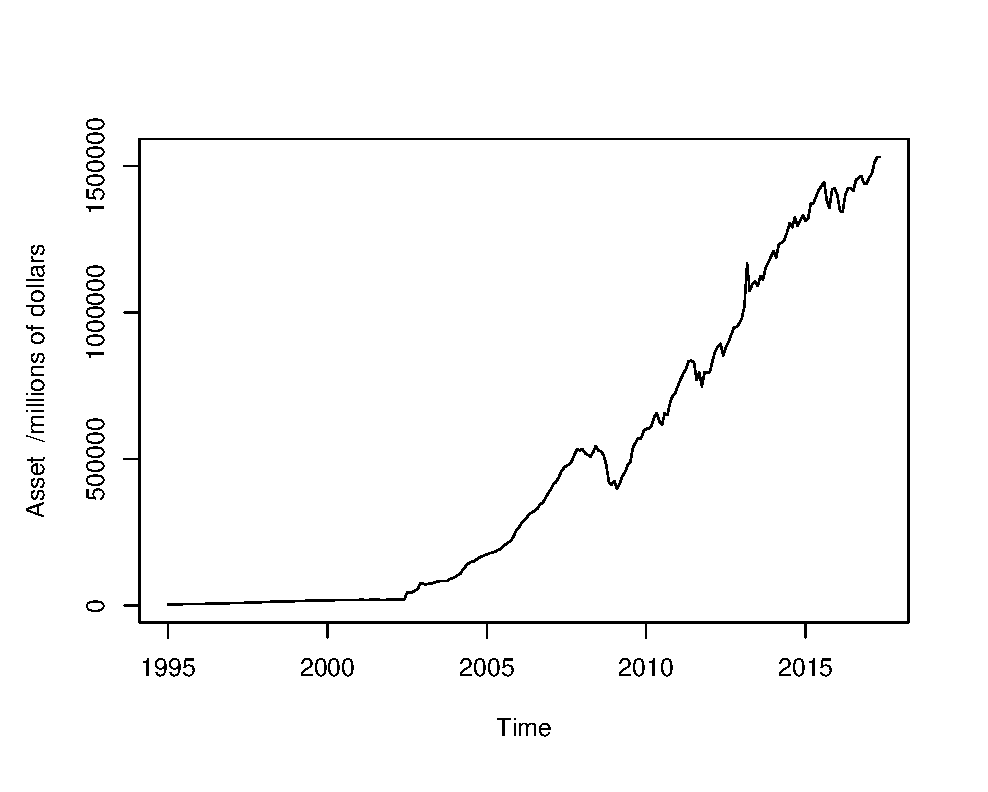
\includegraphics[width=0.5\textwidth]{pic/ast.eps}
    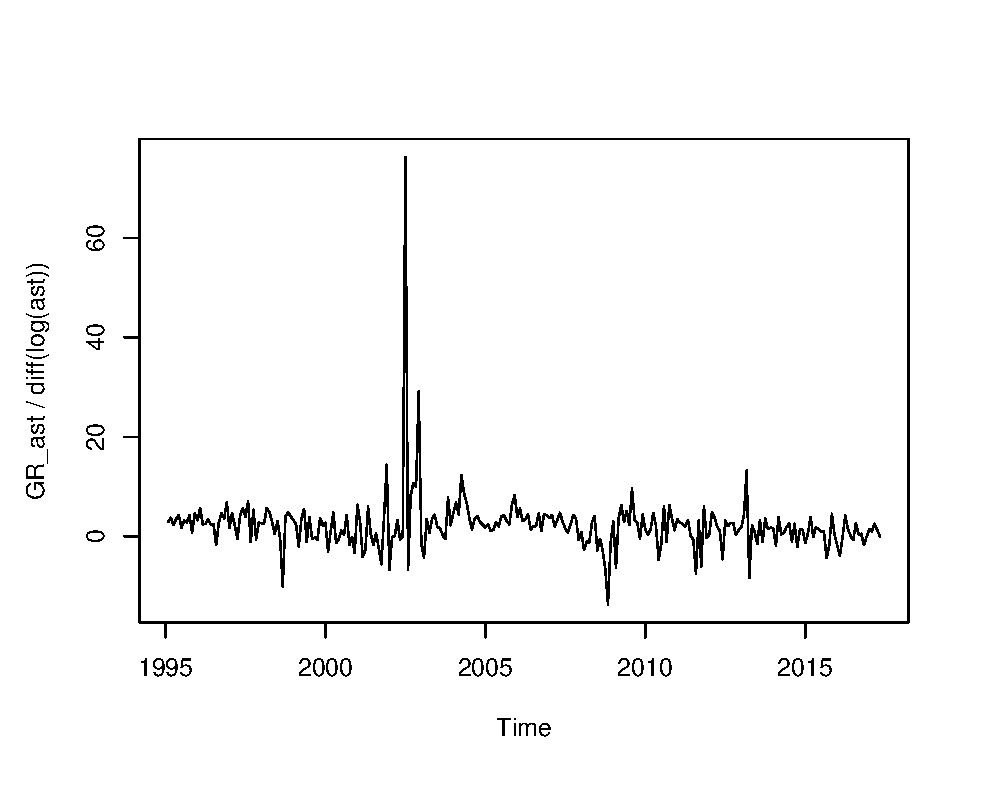
\includegraphics[width=0.5\textwidth]{pic/gr_ast.eps}
\end{figure}

\begin{figure}[h!]
    % \label{fg:test1}
    \begin{multicols}{2}  
        \begin{minipage}[h]{0.5\textwidth} 
            \centering   
            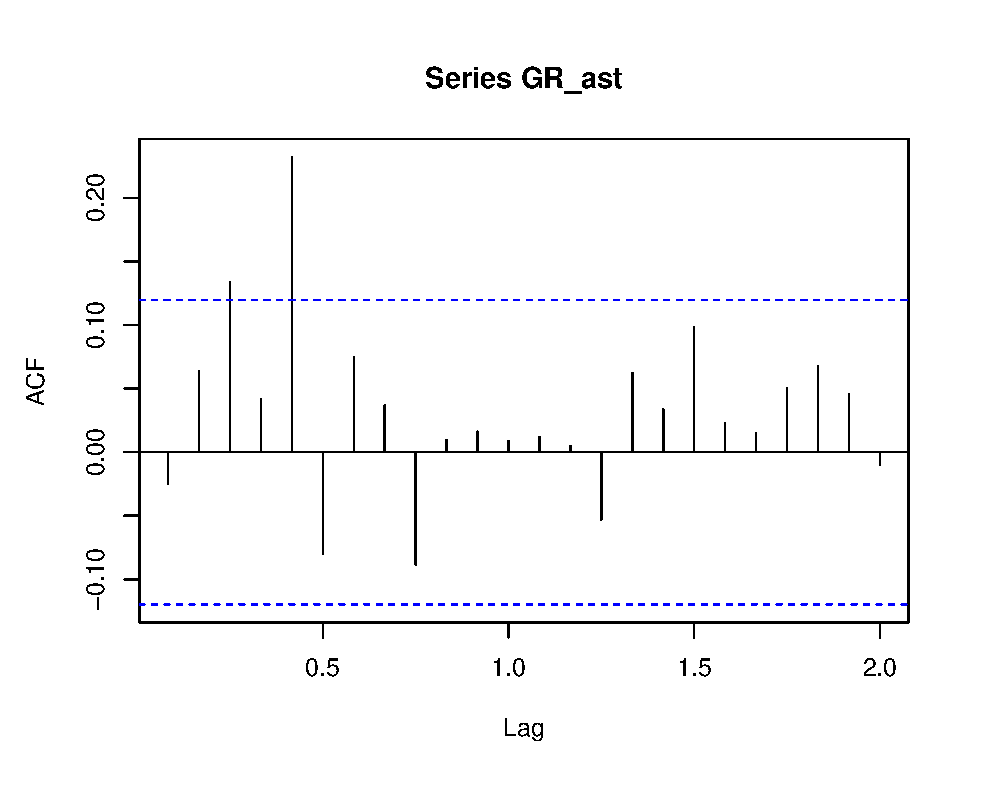
\includegraphics[width=1\textwidth]{pic/acf(gr_ast)}   
            \subcaption{ACF of GR\_ast}   \label{fig:apegrast:a}   
        \end{minipage}
        \begin{minipage}[h]{0.5\textwidth}   
            \centering   
            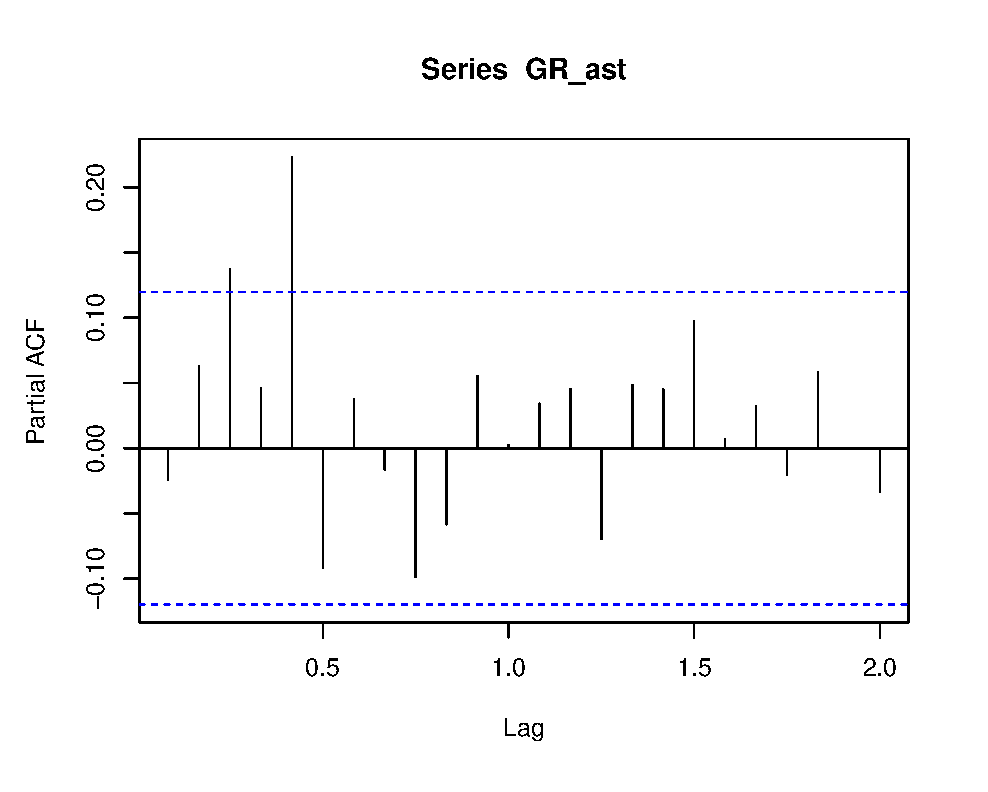
\includegraphics[width=1\textwidth]{pic/pacf(gr_ast)}   
            \subcaption{PACF of GR\_ast}   
            \label{fig:pierce:b}   
        \end{minipage}


        \begin{minipage}[h]{0.5\textwidth} 
            \centering   
            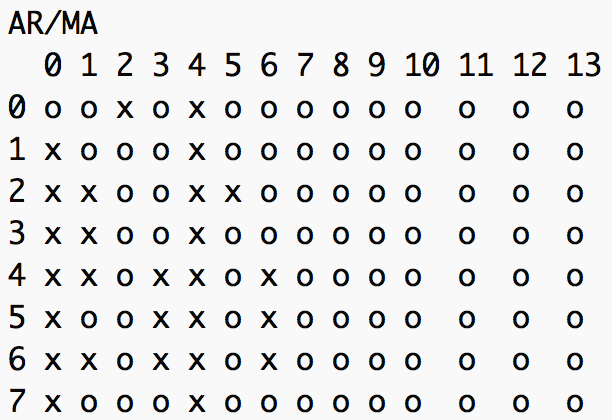
\includegraphics[width=1\textwidth]{pic/eacf(gr_ast)}   
            \subcaption{EACF of GR\_ast}   \label{fig:apegrast:c}   
        \end{minipage}
        \begin{minipage}[h]{0.5\textwidth} 
            \centering   
            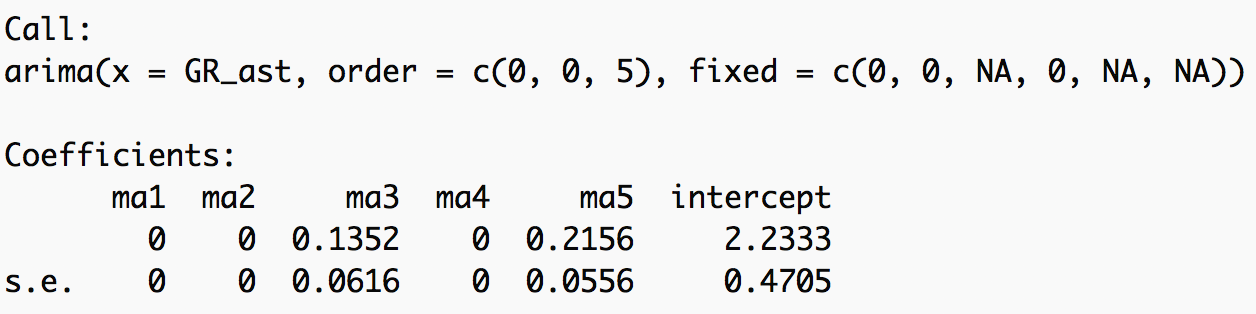
\includegraphics[width=1\textwidth]{pic/ma5}   
            \subcaption{MA Model}   \label{fig:apegrast:d}   
        \end{minipage}    
        \caption{识别MA(q)模型} \label{fig:apegrast}
    \end{multicols}
\end{figure}

% 残差估计结果
% 残差平方估计结果
\begin{figure}[h!]
    \caption{模型诊断} \label{fg:check}
    \begin{multicols}{2}
        \begin{minipage}[h]{0.5\textwidth} 
            \centering   
            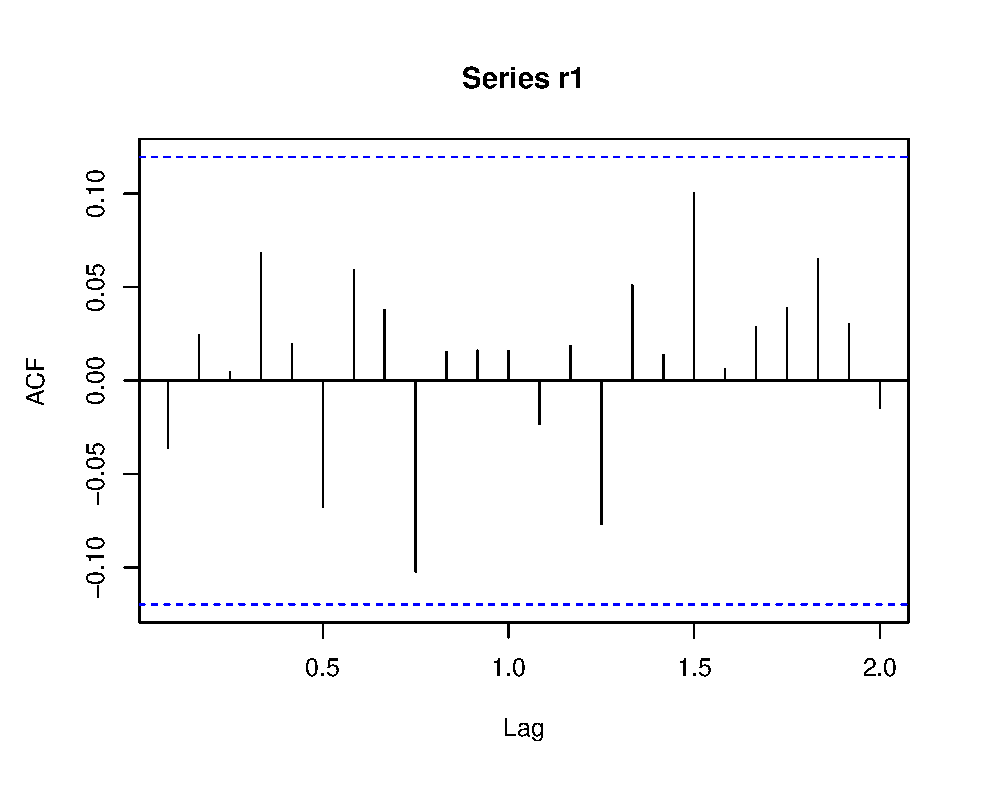
\includegraphics[width=1\textwidth]{pic/acfr1.eps}   
            \subcaption{ACF of residuals}   \label{fig:acfr1}   
        \end{minipage}
        \begin{minipage}[h]{0.5\textwidth}   
            \centering   
            % 
            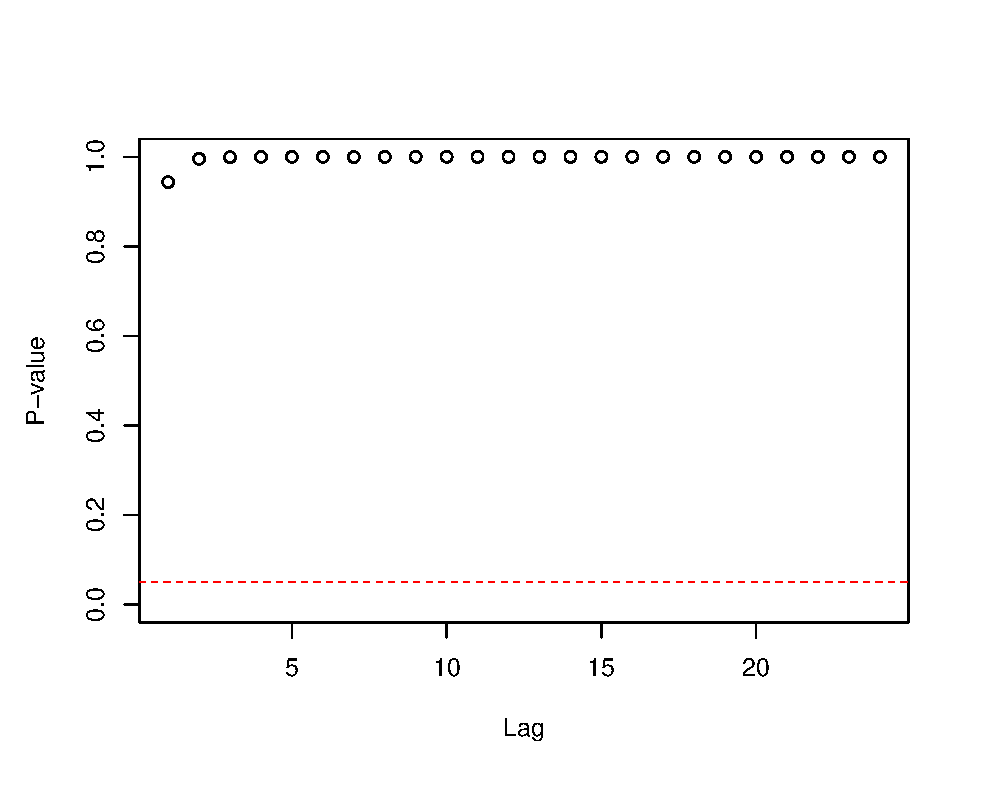
\includegraphics[width=1\textwidth]{pic/mc_gr_ast.eps} 
            \subcaption{McLeod.Li.test of residuals}   
            \label{fig:mcgrast}   
        \end{minipage}
    \end{multicols}
\end{figure}
% 异常值诊断情况
\begin{figure}[h!]
    \caption{异常值诊断}
    \centering
    % 异常值诊断1
    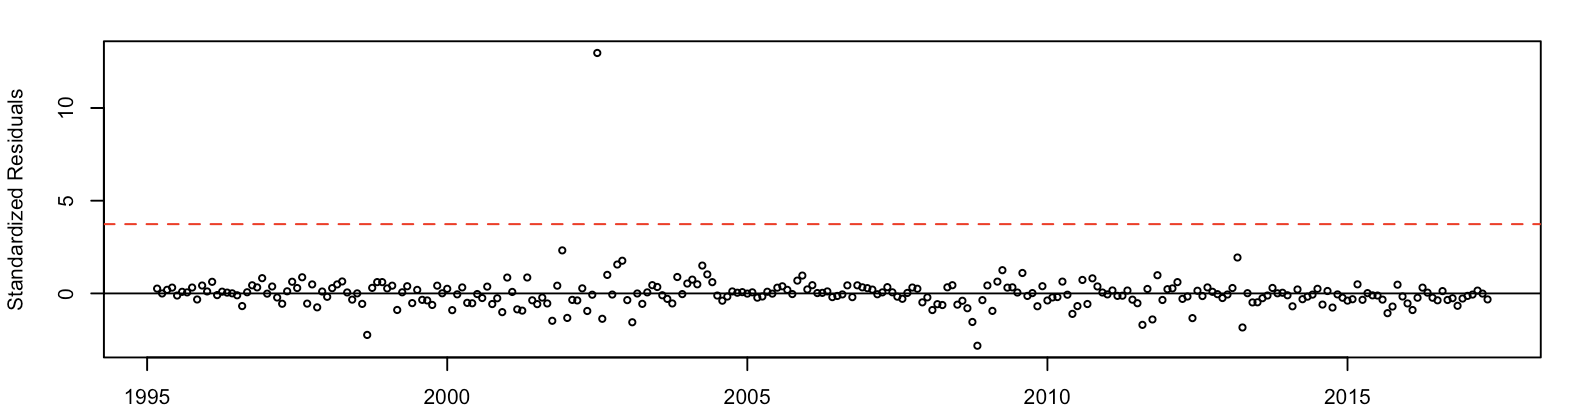
\includegraphics[width=0.8\linewidth]{pic/srgr_ast}
    \subcaption{Standardized Residuals of MA Model for GR\_ast }
    \label{fig:srgrast}
    % \end{figure}
    % \begin{figure}
    % \centering
    % 异常值诊断2
    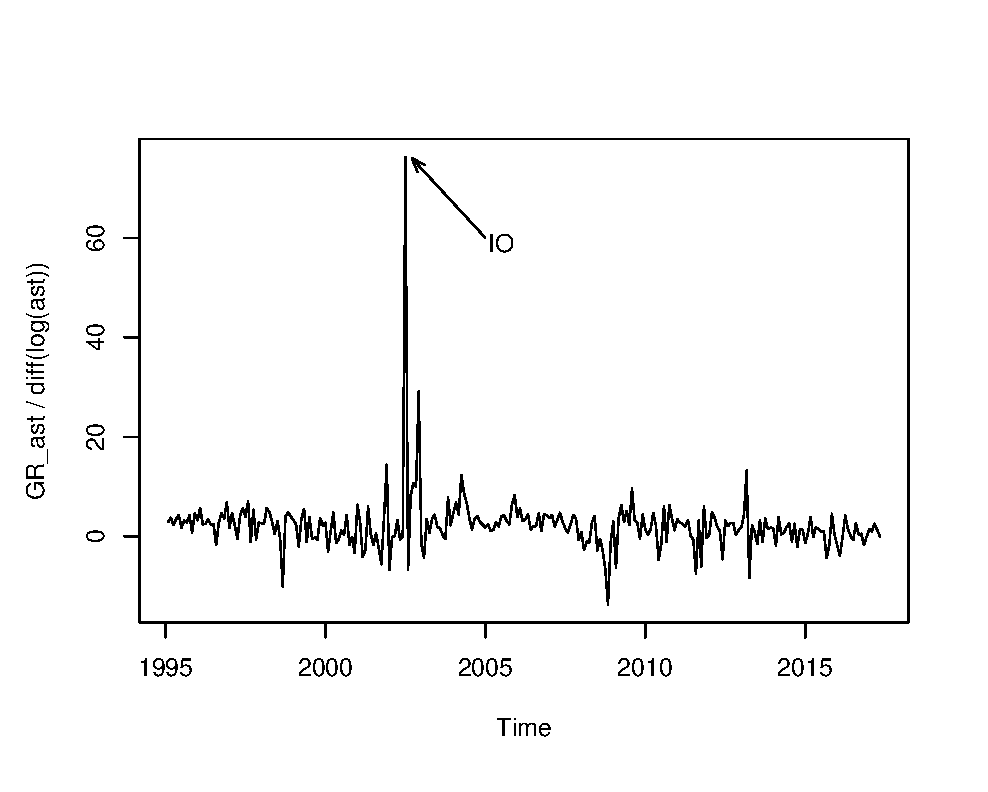
\includegraphics[width=0.5\linewidth]{pic/io}
    \subcaption{Detected outlier}
    \label{fig:io}
\end{figure}
\begin{figure}
    \caption{调整后的增长率序列}
    \centering
    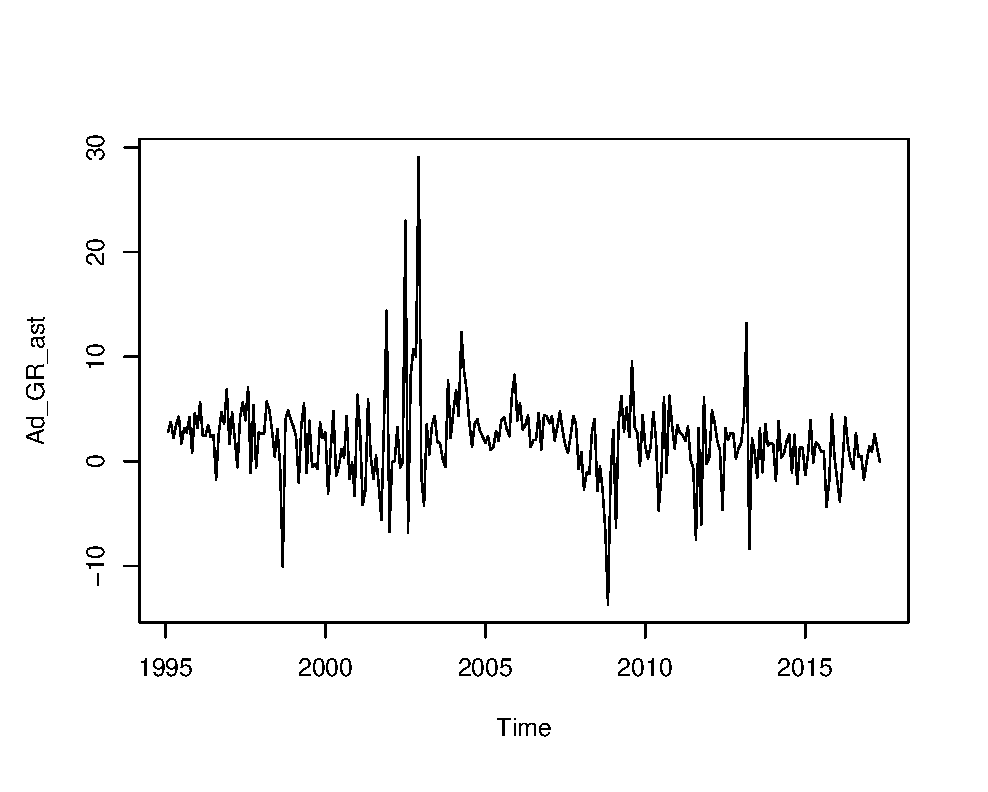
\includegraphics[width=0.5\linewidth]{pic/adgrast}
    \label{fig:adgrast}
\end{figure}
% 调整后的存在Garch效应的原模型
\begin{figure}[h!]
    % \centering
    \begin{center}
    % 
    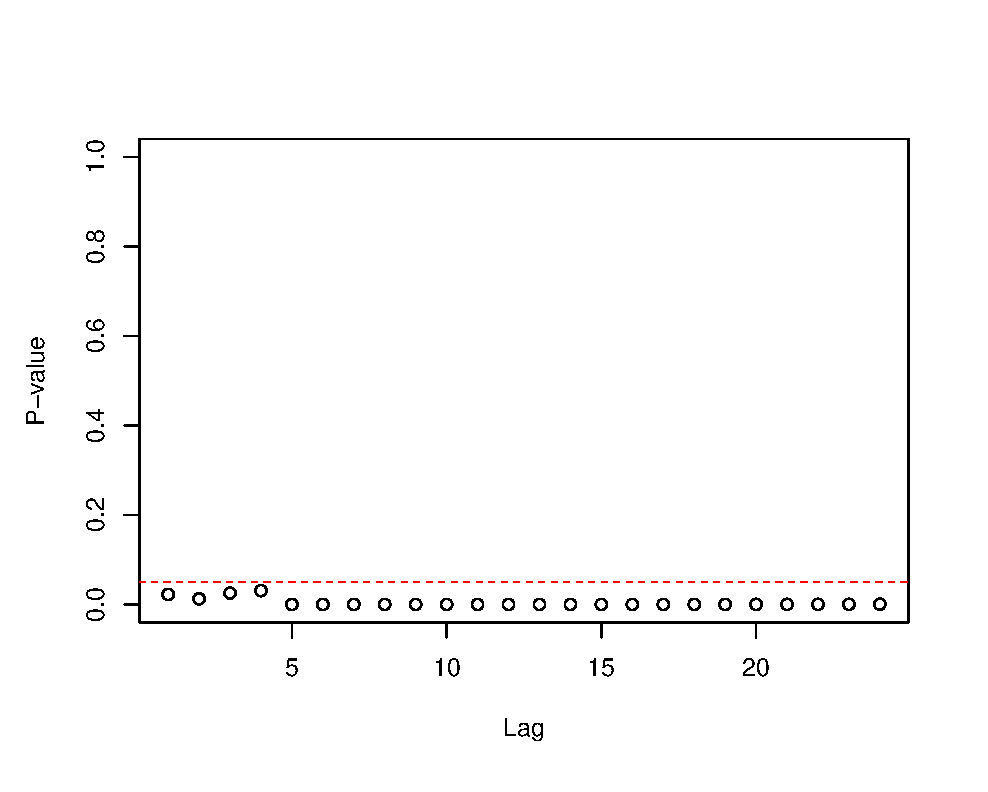
\includegraphics[width=0.5\linewidth]{pic/mcr2}
    \caption{McLeod.Li.test for the residuals of adjusted series}
    \label{fig:mcr2}
    \end{center}
\end{figure}
\begin{figure}[h!]
    % \centering
    \begin{center}
    % ARMA(0,5)-GARCH(0,1)估计结果
    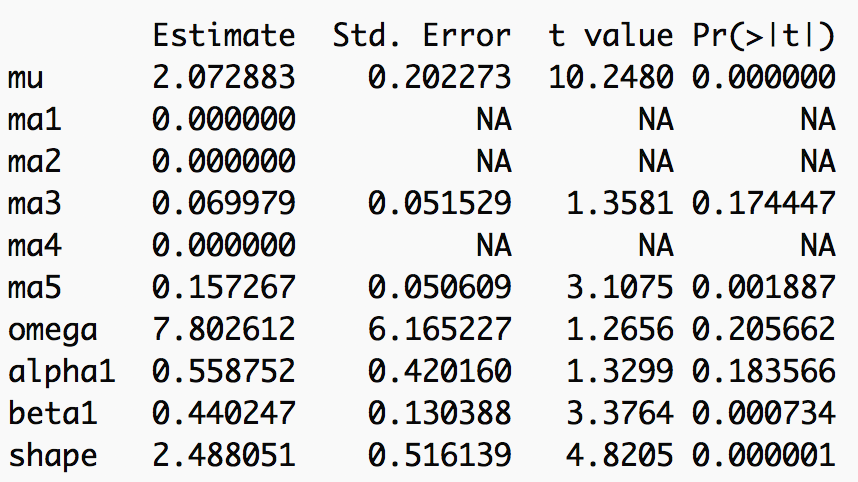
\includegraphics[width=0.7\linewidth]{pic/astgarch}
    \caption{Parameters and t-value,  Distribution    : std }
    \label{fig:astg}
    \end{center}
\end{figure}

\begin{figure}[h!]
    \caption{FOF基金市场与养老金市场} 
    \label{fg:3}
    % 两个市场的趋势图像
    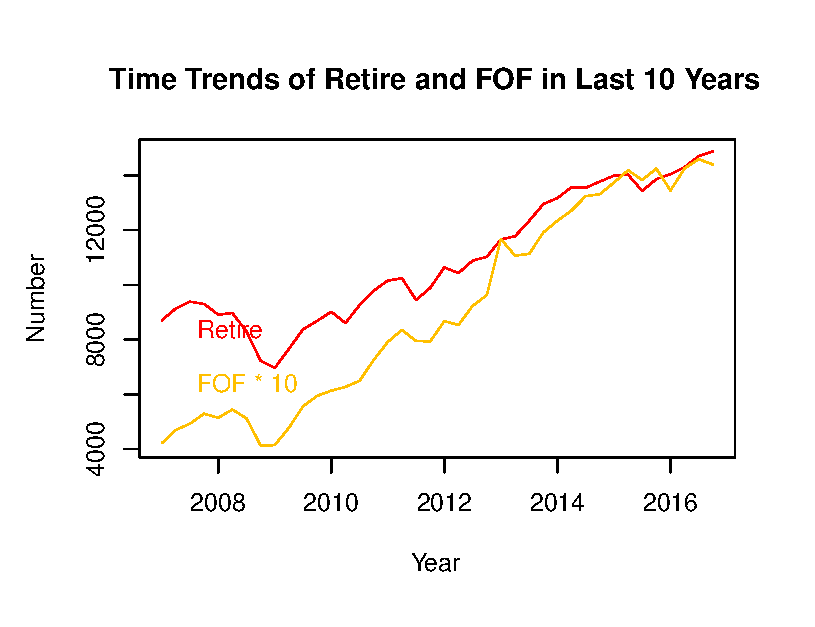
\includegraphics[width=0.5\textwidth]{3-0-1.eps}
    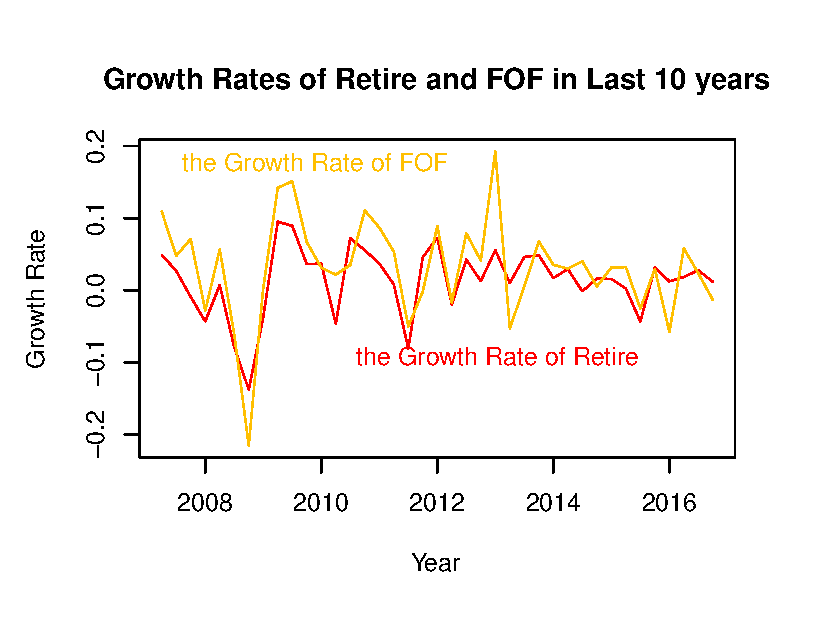
\includegraphics[width=0.5\textwidth]{3-0-2.eps}
\end{figure}

\section{附表}
% OLS回归结果表格
\begin{table}[h!]
    \centering
    \caption{OLS估计结果}
    \label{tb:ols}
    \begin{tabular}{l | llll}
        Coefficients: &            &            &         &                     \\
                      & Estimate   & Std. Error & t value & Pr(\textgreater|t|) \\  \hline
        (Intercept)   & -7.552e+02 & 5.632e+01  & -13.41  & 5.51e-16 ***        \\
        Retire        & 1.524e-01  & 5.042e-03  & 30.22   & \textless 2e-16 ***
    \end{tabular}
\end{table}

% 残差具有平稳性
\begin{table}[h!]
    \centering
    \caption{OLS估计残差的单位根检验}
    \label{tb:adf}
    \begin{tabular}{l | llll}
        Tests        & ADF-Test       & KPSS-Test      & PP-Test               \\  \hline
        Statistics   & -3.1799 (<1pct & 0.2674(<10pct) & -10.0379 (<Z-tau)  
    \end{tabular}
\end{table}

\begin{table}[h!]
    \centering
    \caption{误差修正模型估计结果}
    \label{tb:ecm}
    \begin{tabular}{l | llll}
        Coefficients: &          &            &         &                     \\
                      & Estimate & Std. Error & t value & Pr(\textgreater|t|) \\  \hline
        (Intercept)   & 22.13335 & 11.14436   & 1.986   & 0.0573              \\
        L(y, 1)       & -0.46108 & 0.19994    & -2.306  & 0.029 *             \\
        L(y, 2)       & -0.01601 & 0.12908    & -0.124  & 0.9022              \\
        L(y, 3)       & -0.03563 & 0.12999    & -0.274  & 0.7861              \\
        L(y, 4)       & -0.02875 & 0.13862    & -0.207  & 0.8373              \\
        L(x, 1)       & 0.05842  & 0.02549    & 2.292   & 0.03 *              \\
        L(x, 0)       & 0.09517  & 0.01852    & 5.138   & 0.000021 ***        \\
        L(r, 1)       & -0.38373 & 0.16855    & -2.277  & 0.0309 *           
    \end{tabular}
\end{table}

\section{数据}
\subsection{美国基金中基金市场的规模}
\begin{center}
\begin{longtable}{rr|rr|rr}
\caption{1995年1月至2017年5月美国基金中基金市场的规模\label{tab:fof}}\\
\hline\hline
    \multicolumn{1}{c}{\multirow{2}[0]{*}{\textbf{时间}}} & \multicolumn{1}{c|}{\textbf{资产}} & \multicolumn{1}{c}{\multirow{2}[0]{*}{\textbf{时间}}} & \multicolumn{1}{c|}{\textbf{资产}} & \multicolumn{1}{c}{\multirow{2}[0]{*}{\textbf{时间}}} & \multicolumn{1}{c}{\textbf{资产}} \\
          & \multicolumn{1}{c|}{\textbf{(百万美元)}} &       & \multicolumn{1}{c|}{\textbf{(百万美元)}} &       & \multicolumn{1}{c}{\textbf{(百万美元)}} \\
\hline
\endfirsthead
\multicolumn{6}{c}%
{\tablename\ \thetable\ -- \textit{接上页}} \\
\hline
    \multicolumn{1}{c}{\multirow{2}[0]{*}{\textbf{时间}}} & \multicolumn{1}{c|}{\textbf{资产}} & \multicolumn{1}{c}{\multirow{2}[0]{*}{\textbf{时间}}} & \multicolumn{1}{c|}{\textbf{资产}} & \multicolumn{1}{c}{\multirow{2}[0]{*}{\textbf{时间}}} & \multicolumn{1}{c}{\textbf{资产}} \\
          & \multicolumn{1}{c|}{\textbf{(百万美元)}} &       & \multicolumn{1}{c|}{\textbf{(百万美元)}} &       & \multicolumn{1}{c}{\textbf{(百万美元)}} \\
\hline
\endhead
\hline \multicolumn{6}{r}{\textit{接下页}} \\
\endfoot
\hline\hline \multicolumn{6}{r}{\textit{数据来源: bloomberg}}
\endlastfoot
    1995/01 & 3891.54 & 1995/02 & 4004.15 & 1995/03 & 4157.77 \\
    1995/04 & 4251.60 & 1995/05 & 4402.44 & 1995/06 & 4593.91 \\
    1995/07 & 4672.64 & 1995/08 & 4823.46 & 1995/09 & 4958.94 \\
    1995/10 & 5171.76 & 1995/11 & 5213.18 & 1995/12 & 5457.18 \\
    1996/01 & 5633.96 & 1996/02 & 5960.12 & 1996/03 & 6106.85 \\
    1996/04 & 6257.97 & 1996/05 & 6480.18 & 1996/06 & 6632.46 \\
    1996/07 & 6800.38 & 1996/08 & 6682.34 & 1996/09 & 6865.76 \\
    1996/10 & 7197.85 & 1996/11 & 7459.89 & 1996/12 & 7989.89 \\
    1997/01 & 8123.58 & 1997/02 & 8514.52 & 1997/03 & 8699.14 \\
    1997/04 & 8649.68 & 1997/05 & 9020.01 & 1997/06 & 9543.86 \\
    1997/07 & 9925.52 & 1997/08 & 10648.88 & 1997/09 & 10530.58 \\
    1997/10 & 11112.78 & 1997/11 & 11044.41 & 1997/12 & 11352.39 \\
    1998/01 & 11655.81 & 1998/02 & 11963.02 & 1998/03 & 12664.41 \\
    1998/04 & 13294.74 & 1998/05 & 13683.06 & 1998/06 & 13746.65 \\
    1998/07 & 14179.25 & 1998/08 & 14128.49 & 1998/09 & 12777.88 \\
    1998/10 & 13300.41 & 1998/11 & 13964.41 & 1998/12 & 14532.98 \\
    1999/01 & 15022.44 & 1999/02 & 15376.77 & 1999/03 & 15066.40 \\
    1999/04 & 15608.80 & 1999/05 & 16495.46 & 1999/06 & 16311.59 \\
    1999/07 & 16957.58 & 1999/08 & 16863.42 & 1999/09 & 16819.18 \\
    1999/10 & 16701.55 & 1999/11 & 17332.58 & 1999/12 & 17721.58 \\
    2000/01 & 18214.94 & 2000/02 & 17662.49 & 2000/03 & 17873.37 \\
    2000/04 & 18751.00 & 2000/05 & 18496.00 & 2000/06 & 18396.02 \\
    2000/07 & 18612.33 & 2000/08 & 18678.35 & 2000/09 & 19502.83 \\
    2000/10 & 19172.91 & 2000/11 & 19151.47 & 2000/12 & 18528.61 \\
    2001/01 & 19749.24 & 2001/02 & 20338.12 & 2001/03 & 19507.07 \\
    2001/04 & 18978.33 & 2001/05 & 20144.45 & 2001/06 & 20245.34 \\
    2001/07 & 19905.22 & 2001/08 & 20014.13 & 2001/09 & 19558.66 \\
    2001/10 & 18492.07 & 2001/11 & 19243.60 & 2001/12 & 22221.82 \\
    2002/01 & 20769.81 & 2002/02 & 20746.55 & 2002/03 & 20755.45 \\
    2002/04 & 21449.55 & 2002/05 & 21321.43 & 2002/06 & 21301.30 \\
    2002/07 & 45669.03 & 2002/08 & 42665.45 & 2002/09 & 46329.04 \\
    2002/10 & 51587.31 & 2002/11 & 57018.59 & 2002/12 & 76280.67 \\
    2003/01 & 75090.64 & 2003/02 & 71979.21 & 2003/03 & 74544.03 \\
    2003/04 & 75032.41 & 2003/05 & 77723.33 & 2003/06 & 81166.19 \\
    2003/07 & 82694.96 & 2003/08 & 84115.64 & 2003/09 & 84286.23 \\
    2003/10 & 83845.05 & 2003/11 & 90622.28 & 2003/12 & 92661.04 \\
    2004/01 & 97158.40 & 2004/02 & 104011.11 & 2004/03 & 108635.58 \\
    2004/04 & 122895.62 & 2004/05 & 133983.55 & 2004/06 & 143331.71 \\
    2004/07 & 148663.38 & 2004/08 & 150728.16 & 2004/09 & 156230.53 \\
    2004/10 & 162639.36 & 2004/11 & 167402.90 & 2004/12 & 171383.94 \\
    2005/01 & 174442.90 & 2005/02 & 178663.61 & 2005/03 & 180644.12 \\
    2005/04 & 183032.82 & 2005/05 & 188376.19 & 2005/06 & 192123.44 \\
    2005/07 & 199859.87 & 2005/08 & 208480.39 & 2005/09 & 215081.04 \\
    2005/10 & 220273.78 & 2005/11 & 234997.47 & 2005/12 & 255266.06 \\
    2006/01 & 265454.38 & 2006/02 & 280590.70 & 2006/03 & 289272.48 \\
    2006/04 & 299346.94 & 2006/05 & 312759.22 & 2006/06 & 317089.00 \\
    2006/07 & 323568.98 & 2006/08 & 330218.35 & 2006/09 & 345766.22 \\
    2006/10 & 349620.43 & 2006/11 & 365517.94 & 2006/12 & 381525.97 \\
    2007/01 & 395654.18 & 2007/02 & 413001.92 & 2007/03 & 421266.16 \\
    2007/04 & 435453.75 & 2007/05 & 456568.17 & 2007/06 & 469966.94 \\
    2007/07 & 477194.84 & 2007/08 & 480902.06 & 2007/09 & 493065.61 \\
    2007/10 & 514898.91 & 2007/11 & 533376.36 & 2007/12 & 529529.30 \\
    2008/01 & 534289.55 & 2008/02 & 520191.05 & 2008/03 & 514646.96 \\
    2008/04 & 508470.37 & 2008/05 & 523082.91 & 2008/06 & 544725.97 \\
    2008/07 & 529515.72 & 2008/08 & 526861.80 & 2008/09 & 512458.99 \\
    2008/10 & 479500.51 & 2008/11 & 418175.57 & 2008/12 & 413135.16 \\
    2009/01 & 425735.13 & 2009/02 & 399602.82 & 2009/03 & 414628.09 \\
    2009/04 & 441387.68 & 2009/05 & 454104.29 & 2009/06 & 478017.71 \\
    2009/07 & 489189.85 & 2009/08 & 538315.04 & 2009/09 & 556143.45 \\
    2009/10 & 571690.68 & 2009/11 & 569009.49 & 2009/12 & 594713.21 \\
    2010/01 & 603296.68 & 2010/02 & 604997.72 & 2010/03 & 613747.34 \\
    2010/04 & 643478.26 & 2010/05 & 657422.41 & 2010/06 & 627196.83 \\
    2010/07 & 618079.94 & 2010/08 & 656942.36 & 2010/09 & 649672.88 \\
    2010/10 & 691727.30 & 2010/11 & 717014.97 & 2010/12 & 725812.87 \\
    2011/01 & 751328.49 & 2011/02 & 772202.43 & 2011/03 & 791899.00 \\
    2011/04 & 807483.61 & 2011/05 & 834704.22 & 2011/06 & 835778.39 \\
    2011/07 & 830000.85 & 2011/08 & 769909.22 & 2011/09 & 794900.02 \\
    2011/10 & 748423.04 & 2011/11 & 795681.22 & 2011/12 & 793597.63 \\
    2012/01 & 796472.81 & 2012/02 & 836033.37 & 2012/03 & 867648.22 \\
    2012/04 & 884599.71 & 2012/05 & 893903.72 & 2012/06 & 853352.89 \\
    2012/07 & 880810.17 & 2012/08 & 899012.82 & 2012/09 & 923559.21 \\
    2012/10 & 948199.53 & 2012/11 & 950534.35 & 2012/12 & 962415.61 \\
    2013/01 & 979779.23 & 2013/02 & 1022456.88 & 2013/03 & 1167128.29 \\
    2013/04 & 1073323.00 & 2013/05 & 1097449.88 & 2013/06 & 1107170.36 \\
    2013/07 & 1089874.24 & 2013/08 & 1124873.00 & 2013/09 & 1113023.58 \\
    2013/10 & 1153404.90 & 2013/11 & 1170515.85 & 2013/12 & 1191252.26 \\
    2014/01 & 1210088.64 & 2014/02 & 1187520.60 & 2014/03 & 1234096.87 \\
    2014/04 & 1238799.16 & 2014/05 & 1247947.58 & 2014/06 & 1271898.35 \\
    2014/07 & 1304877.84 & 2014/08 & 1290804.96 & 2014/09 & 1324078.57 \\
    2014/10 & 1295844.43 & 2014/11 & 1313867.10 & 2014/12 & 1331161.52 \\
    2015/01 & 1313628.87 & 2015/02 & 1321029.56 & 2015/03 & 1373800.97 \\
    2015/04 & 1372278.97 & 2015/05 & 1397090.52 & 2015/06 & 1418694.42 \\
    2015/07 & 1431861.66 & 2015/08 & 1445206.70 & 2015/09 & 1383349.54 \\
    2015/10 & 1357479.17 & 2015/11 & 1420458.98 & 2015/12 & 1424948.06 \\
    2016/01 & 1399192.81 & 2016/02 & 1346345.30 & 2016/03 & 1344888.45 \\
    2016/04 & 1402333.30 & 2016/05 & 1424562.38 & 2016/06 & 1425313.57 \\
    2016/07 & 1414559.58 & 2016/08 & 1453163.33 & 2016/09 & 1459183.73 \\
    2016/10 & 1466733.52 & 2016/11 & 1440816.65 & 2016/12 & 1439637.04 \\
    2017/01 & 1460271.42 & 2017/02 & 1473791.88 & 2017/03 & 1512170.81 \\
    2017/04 & 1531286.24 & 2017/05 & 1531106.44 &       &  \\
\end{longtable}
\end{center}

\subsection{美国退休养老资产规模}
\begin{footnotesize}
\begin{center}
\begin{longtable}{rrrrrrrr}
  \caption{2007年1季度至2016年4季度美国退休养老资产规模~~(单位:十亿美元)\label{tab:retire}}\\
\hline\hline
    \multirow{2}[0]{*}{\textbf{Time}} & \multirow{2}[0]{*}{\textbf{IRAs}} & \textbf{\tiny DC} & \textbf{\tiny Private-Sector} & \textbf{\tiny Government} & \textbf{\tiny Federal} & \multirow{2}[0]{*}{\textbf{Annuities}} & \multirow{2}[0]{*}{\textbf{Total}} \\
          &       & \textbf{\tiny Plans} & \textbf{\tiny DB Plans} & \textbf{\tiny DB Plans} & \textbf{\tiny DB Plans} &       &  \\
\hline
\endfirsthead
\multicolumn{8}{c}%
{\tablename\ \thetable\ -- \textit{接上页}} \\
\hline
    \multirow{2}[0]{*}{\textbf{Time}} & \multirow{2}[0]{*}{\textbf{IRAs}} & \textbf{\tiny DC} & \textbf{\tiny Private-Sector} & \textbf{\tiny Government} & \textbf{\tiny Federal} & \multirow{2}[0]{*}{\textbf{Annuities}} & \multirow{2}[0]{*}{\textbf{Total}} \\
          &       & \textbf{\tiny Plans} & \textbf{\tiny DB Plans} & \textbf{\tiny DB Plans} & \textbf{\tiny DB Plans} &       &  \\
\hline
\endhead
\hline \multicolumn{8}{r}{\textit{接下页}} \\
\endfoot
\hline\hline \multicolumn{8}{r}{\textit{数据来源: Investment Company Institute (ICI)}}
\endlastfoot
    2007:Q1 & 4340  & 4360  & 2520  & 3161  & 930   & 1431  & 16742  \\
    2007:Q2 & 4605  & 4535  & 2675  & 3308  & 920   & 1488  & 17531  \\
    2007:Q3 & 4775  & 4614  & 2685  & 3352  & 936   & 1516  & 17878  \\
    2007:Q4 & 4748  & 4555  & 2646  & 3296  & 978   & 1507  & 17730  \\
    2008:Q1 & 4555  & 4356  & 2515  & 3120  & 961   & 1442  & 16948  \\
    2008:Q2 & 4580  & 4396  & 2495  & 3132  & 967   & 1432  & 17002  \\
    2008:Q3 & 4225  & 4069  & 2340  & 2944  & 984   & 1369  & 15931  \\
    2008:Q4 & 3681  & 3547  & 1979  & 2466  & 1033  & 1239  & 13946  \\
    2009:Q1 & 3536  & 3429  & 1840  & 2288  & 1009  & 1193  & 13296  \\
    2009:Q2 & 3925  & 3736  & 1990  & 2407  & 1015  & 1275  & 14347  \\
    2009:Q3 & 4325  & 4053  & 2155  & 2619  & 1032  & 1363  & 15546  \\
    2009:Q4 & 4488  & 4200  & 2228  & 2728  & 1095  & 1397  & 16137  \\
    2010:Q1 & 4644  & 4373  & 2315  & 2833  & 1079  & 1439  & 16683  \\
    2010:Q2 & 4405  & 4204  & 2210  & 2623  & 1081  & 1392  & 15915  \\
    2010:Q3 & 4757  & 4500  & 2345  & 2762  & 1099  & 1482  & 16944  \\
    2010:Q4 & 5029  & 4758  & 2481  & 2954  & 1161  & 1557  & 17941  \\
    2011:Q1 & 5255  & 4903  & 2545  & 3049  & 1147  & 1606  & 18504  \\
    2011:Q2 & 5315  & 4927  & 2535  & 3004  & 1155  & 1614  & 18550  \\
    2011:Q3 & 4910  & 4538  & 2440  & 2673  & 1165  & 1512  & 17238  \\
    2011:Q4 & 5153  & 4738  & 2525  & 2838  & 1230  & 1574  & 18057  \\
    2012:Q1 & 5550  & 5089  & 2685  & 3048  & 1214  & 1672  & 19259  \\
    2012:Q2 & 5450  & 4981  & 2640  & 2951  & 1220  & 1635  & 18878  \\
    2012:Q3 & 5700  & 5186  & 2723  & 3025  & 1239  & 1688  & 19562  \\
    2012:Q4 & 5785  & 5242  & 2709  & 2998  & 1270  & 1705  & 19709  \\
    2013:Q1 & 6123  & 5535  & 2790  & 3190  & 1282  & 1756  & 20675  \\
    2013:Q2 & 6189  & 5587  & 2775  & 3240  & 1287  & 1758  & 20836  \\
    2013:Q3 & 6487  & 5848  & 2808  & 3349  & 1301  & 1816  & 21609  \\
    2013:Q4 & 6819  & 6132  & 2892  & 3549  & 1370  & 1886  & 22648  \\
    2014:Q1 & 6961  & 6212  & 2910  & 3559  & 1357  & 1899  & 22898  \\
    2014:Q2 & 7215  & 6352  & 2968  & 3641  & 1360  & 1939  & 23475  \\
    2014:Q3 & 7182  & 6367  & 2949  & 3630  & 1378  & 1925  & 23431  \\
    2014:Q4 & 7292  & 6480  & 3003  & 3730  & 1438  & 1954  & 23896  \\
    2015:Q1 & 7445  & 6547  & 3003  & 3756  & 1417  & 1976  & 24145  \\
    2015:Q2 & 7504  & 6522  & 2972  & 3772  & 1419  & 1979  & 24168  \\
    2015:Q3 & 7133  & 6298  & 2828  & 3551  & 1439  & 1910  & 23160  \\
    2015:Q4 & 7329  & 6537  & 2870  & 3664  & 1512  & 1954  & 23866  \\
    2016:Q1 & 7400  & 6639  & 2863  & 3665  & 1497  & 1976  & 24041  \\
    2016:Q2 & 7527  & 6775  & 2876  & 3714  & 1497  & 2004  & 24392  \\
    2016:Q3 & 7767  & 6938  & 2916  & 3813  & 1515  & 2045  & 24992  \\
    2016:Q4 & 7850  & 7028  & 2946  & 3861  & 1595  & 2049  & 25330  \\
\end{longtable}
\end{center}
\end{footnotesize} 
% \end{appendices}
\end{document}
